\documentclass[border=10pt]{standalone}
\usepackage{tikz}
\usepackage{amsmath}
\usetikzlibrary{arrows.meta, positioning, fit, backgrounds, calc}

\begin{document}
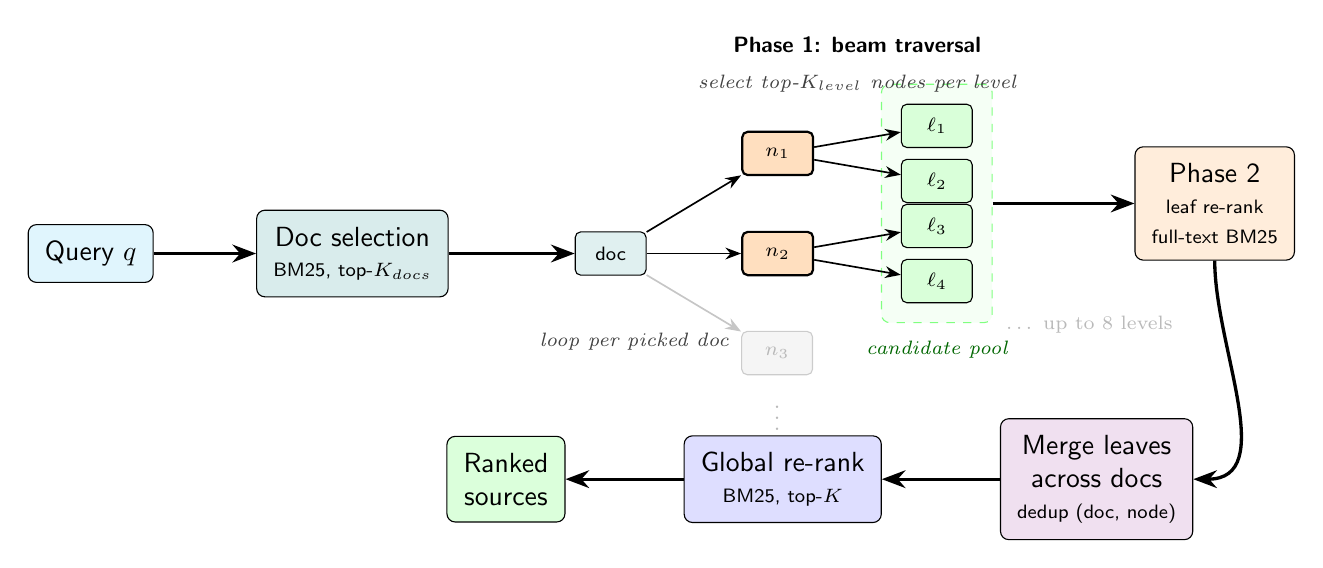
\begin{tikzpicture}[
    font=\small,
    tnode/.style={draw, rounded corners=2pt, minimum width=0.9cm, minimum height=0.55cm,
                  font=\scriptsize\sffamily, align=center},
    sel/.style={tnode, fill=orange!25, line width=0.8pt},
    pruned/.style={tnode, fill=gray!8, text=gray!55, draw=gray!40},
    leaf/.style={tnode, fill=green!15},
    box/.style={draw, rounded corners=3pt, align=center, font=\sffamily,
                inner sep=6pt},
    arr/.style={-{Stealth[length=2mm]}, semithick},
    parr/.style={-{Stealth[length=2mm]}, semithick, gray!45},
    flow/.style={-{Stealth[length=3mm]}, very thick},
]

    %==================== QUERY ====================
    \node[box, fill=cyan!12] (q) {Query $q$};

    %==================== STAGE 1 ====================
    \node[box, fill=teal!15, right=1.3cm of q] (docpick)
        {Doc selection\\[-1pt]{\scriptsize BM25, top-$K_{docs}$}};
    \draw[flow] (q) -- (docpick);

    %==================== TREE (Phase 1: beam traversal) ====================
    % root level
    \node[tnode, fill=teal!12, right=1.6cm of docpick] (root) {doc};

    % level 1
    \node[sel, above right=0.7cm and 1.2cm of root] (n1) {$n_1$};
    \node[sel, right=1.2cm of root] (n2) {$n_2$};
    \node[pruned, below right=0.7cm and 1.2cm of root] (n3) {$n_3$};

    \draw[arr] (root) -- (n1);
    \draw[arr] (root) -- (n2);
    \draw[parr] (root) -- (n3);
    \draw[flow] (docpick) -- (root);

    % level 2 (children of selected beam)
    \node[leaf, right=1.1cm of n1, yshift=0.35cm] (l1) {$\ell_1$};
    \node[leaf, right=1.1cm of n1, yshift=-0.35cm] (l2) {$\ell_2$};
    \node[leaf, right=1.1cm of n2, yshift=0.35cm] (l3) {$\ell_3$};
    \node[leaf, right=1.1cm of n2, yshift=-0.35cm] (l4) {$\ell_4$};

    \draw[arr] (n1) -- (l1);
    \draw[arr] (n1) -- (l2);
    \draw[arr] (n2) -- (l3);
    \draw[arr] (n2) -- (l4);

    % implied deeper levels
    \node[font=\footnotesize, text=gray!55, below=0.15cm of n3, yshift=0.1cm] {$\vdots$};
    \node[font=\scriptsize, text=gray!55, right=0.3cm of l4, yshift=-0.55cm]
        {\ldots\ up to 8 levels};

    %==================== Phase 1 label (stacked above tree, clear of all nodes) ====================
    \node[font=\sffamily\bfseries\footnotesize, anchor=south] (p1lab)
        at ($(n1.north)!0.5!(l1.north) + (0,0.7)$) {Phase 1: beam traversal};
    \node[font=\scriptsize\itshape, text=gray!50!black, anchor=north]
        at ([yshift=-1pt]p1lab.south)
        {select top-$K_{level}$ nodes per level};

    %==================== candidate pool fit box ====================
    \begin{scope}[on background layer]
        \node[draw=green!50, dashed, rounded corners=3pt, fill=green!4,
              fit=(l1)(l2)(l3)(l4), inner sep=7pt] (pool) {};
    \end{scope}
    \node[font=\scriptsize\itshape, text=green!40!black, below=0.1cm of pool]
        {candidate pool};

    %==================== per-doc loop annotation (clearly under root) ====================
    \node[font=\scriptsize\itshape, text=gray!50!black, below=0.6cm of root, xshift=0.3cm]
        {loop per picked doc};

    %==================== Phase 2 ====================
    \node[box, fill=orange!14, right=1.8cm of pool, align=center] (rerank)
        {Phase 2\\[-1pt]{\scriptsize leaf re-rank}\\[-1pt]{\scriptsize full-text BM25}};
    \draw[flow] (pool) -- (rerank);

    %==================== MERGE + GLOBAL RERANK (bottom row) ====================
    \node[box, fill=violet!12, below=2.0cm of rerank, xshift=-1.5cm] (merge)
        {Merge leaves\\ across docs\\[-1pt]{\scriptsize dedup (doc, node)}};
    \node[box, fill=blue!13, left=1.5cm of merge] (global)
        {Global re-rank\\[-1pt]{\scriptsize BM25, top-$K$}};
    \node[box, fill=green!14, left=1.5cm of global] (out) {Ranked\\ sources};

    \draw[flow] (rerank.south) to[out=-90, in=0] (merge.east);
    \draw[flow] (merge) -- (global);
    \draw[flow] (global) -- (out);

\end{tikzpicture}
\end{document}